\begin{frame}[allowframebreaks]{Unsupervised Learning - Types}
    \begin{itemize}
        \item \textbf{Cluster Analysis}: 
        \begin{itemize}
            \item For identifying homogenous subgroups of samples.
            \item \textbf{Examples}: K-means, hierarchical clustering, DBSCAN.
        \end{itemize}    
        \item \textbf{Dimensionality Reduction}:
        \begin{itemize}
            \item For finding a low-dimensional representation to characterize and visualize the data.
            \item Reducing the number of features in a dataset while preserving important information.
            \item \textbf{Examples}: PCA, t-SNE, UMAP.
        \end{itemize}
        \item \textbf{Anomaly Detection}: 
        \begin{itemize}
            \item \textbf{Finding outliers in the dataset}: Identifying unusual (rare items, events, or observations) data points that do not conform to expected patterns.
            \item \textbf{Examples}: Isolation Forest, One-Class SVM, Autoencoders.
        \end{itemize}
    \end{itemize}
\end{frame}

\begin{frame}[allowframebreaks]{Clustering}
\begin{columns}
    \begin{column}{0.45\textwidth}
        A set of methods for finding  subgroups within the dataset. 
        \vspace{0.8em}
        \begin{itemize}
            \setlength{\itemsep}{0.5em}
            \item Observations should share  common characteristics within the  same group, but differ across  groups.
            \item Groupings are determined from  attributes of the data itself —  differs from classification.
        \end{itemize}
    \end{column}
    \begin{column}{0.55\textwidth}
        \begin{figure}
            \centering
            \fetchconvertimage{https://miro.medium.com/v2/resize:fit:720/format:webp/0*Jwm3mV92c3qRhqEl.}{images/dul/clustering-example.png}{width=0.95\textwidth,keepaspectratio}
            \caption{Taking a 2 dimensional dataset and separating it into 3 distinct clusters. [\href{https://medium.com/square-corner-blog/so-you-have-some-clusters-now-what-abfd297a575b}{Source}]}
        \end{figure}
    \end{column}
\end{columns}

\framebreak

\begin{algorithm}[H]
\caption{Generic Clustering Algorithm}

\KwIn{Dataset $D = \{x_1, x_2, \dots, x_n\}$, number of clusters $k$}
\KwOut{Cluster assignments for each data point}

\vspace{0.5em}
\textbf{Initialization:} Randomly initialize $k$ cluster centroids or seeds\;

\vspace{0.5em}
\Repeat{convergence or maximum iterations reached}{
    \vspace{0.3em}
    \textbf{Assignment Step:} Assign each data point $x_i$ to the nearest cluster based on a distance metric\;
    
    \vspace{0.3em}
    \textbf{Update Step:} Recompute cluster centroids using current assignments\;
}

\vspace{0.5em}
\Return Final cluster assignments\;
\vspace{0.8em}

\end{algorithm}
\end{frame}

\begin{frame}[allowframebreaks]{Clustering Vs Classification}
\begin{figure}
    \centering
    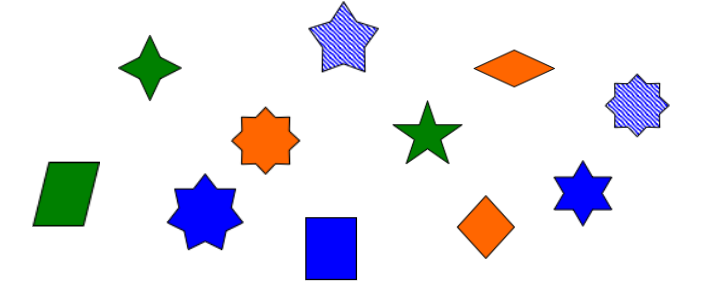
\includegraphics[width=0.8\textwidth,keepaspectratio]{images/dul/sample-clustering-classification.png}
    \caption{Sample data points.}
\end{figure}

\framebreak

\begin{columns}
    \begin{column}{0.5\textwidth}
        \textbf{Classification}
        \begin{itemize}
            \item Labels available
            \item Assigning to known classes
            \item Supervised
        \end{itemize}
        \vspace{1.8em}
        \begin{figure}
            \centering
            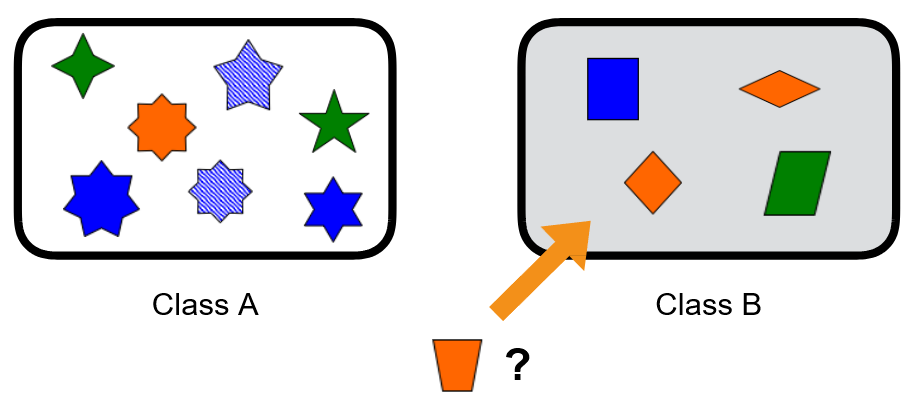
\includegraphics[width=1\textwidth,keepaspectratio]{images/dul/sample-result-classification.png}
            \caption{Classification result.}
        \end{figure}
    \end{column}
    \begin{column}{0.5\textwidth}
        \textbf{Clustering}
        \begin{itemize}
            \item No labels
            \item Grouping based on similarity
            \item Unsupervised
        \end{itemize}
        \vspace{1.8em}
        \begin{figure}
            \centering
            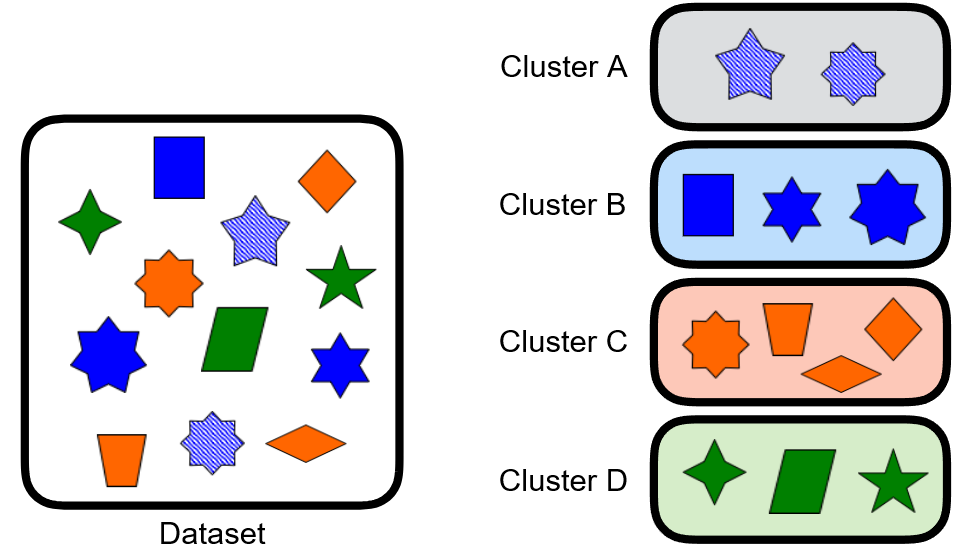
\includegraphics[width=1\textwidth,keepaspectratio]{images/dul/sample-result-clustering.png}
            \caption{Clustering result.}
        \end{figure}
    \end{column}
\end{columns}
\end{frame}

\begin{frame}[allowframebreaks]{Clustering: Types}
    \begin{itemize}
        \item \textbf{Centroid-Based Clustering}: Groups data points based on their proximity to a central point, such as K-means or K-medoids.
        \item \textbf{Hierarchical Clustering}: Builds a hierarchy of clusters using either agglomerative (bottom-up) or divisive (top-down) approaches.
        \item \textbf{Model-Based Clustering}:
        \begin{itemize}
            \item Each cluster is represented by a parametric distribution.
            \item Dataset is a mixture of distributions.
            \item Assumes a probabilistic model for the data and uses statistical methods to identify clusters, such as Gaussian Mixture Models (GMM).
        \end{itemize}
        \item \textbf{Hard Clustering}: 
        \begin{itemize}
            \item Each data point is assigned exclusively to exactly one cluster.
            \item \textbf{Example algorithms}: K-means, Hierarchical clustering.
            \item \textbf{interpretation}: No ambiguity — clusters are crisp and non-overlapping.
        \end{itemize}
        \item \textbf{Soft/Fuzzy Clustering}: 
        \begin{itemize}
            \item Each data point can belong to multiple clusters simultaneously with varying degrees of membership (probabilities or weights).
            \item \textbf{Example algorithms}: Gaussian Mixture Models (GMM), Fuzzy C-means.
            \item \textbf{interpretation}: Reflects uncertainty or mixed membership — clusters can overlap.
        \end{itemize}
    \end{itemize}
\end{frame}

\begin{frame}[allowframebreaks]{Clustering - K-means}
\begin{columns}
    \begin{column}{0.45\textwidth}
        Groups data into $K$ clusters that  satisfy two properties.
        \vspace{0.8em}
        \begin{enumerate}
            \setlength{\itemsep}{0.5em}
            \item Each observation belongs to at least one of the $K$ clusters.
            \item Clusters are non-overlapping.  No observation belongs to more  than one cluster.
        \end{itemize}
    \end{column}
    \begin{column}{0.55\textwidth}
        \begin{figure}
            \centering
            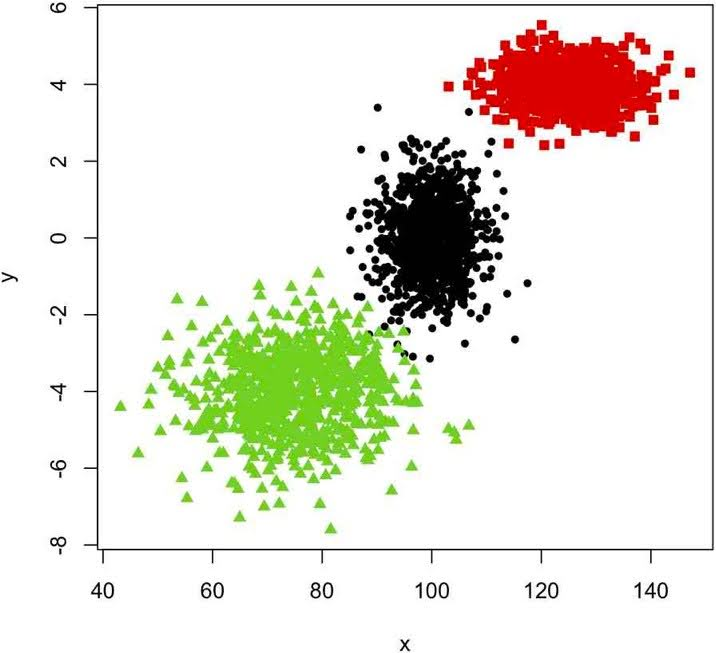
\includegraphics[width=0.95\textwidth,keepaspectratio]{images/dul/kmeans/k-means-example-1.jpg}
            \caption{Clusters.}
        \end{figure}
    \end{column}
\end{columns}

\framebreak

\begin{columns}
    \begin{column}{0.45\textwidth}
    A good clustering is one for which the \textit{within-cluster variation} is as small as possible.

    \vspace{1em}

    Denote each cluster by $C_k$, and let $W(C_k)$ be a measure of the within-cluster variation.

    \vspace{1em}

    K-means aims to solve the following optimization problem:

    \vspace{0.5em}

    \begin{equation}
        \operatorname*{minimise}_{C_1, \ldots, C_k} \left\{ \sum_{k=1}^{K} W(C_k) \right\}
    \end{equation}

    \end{column}
    \begin{column}{0.55\textwidth}
        \begin{figure}
            \centering
            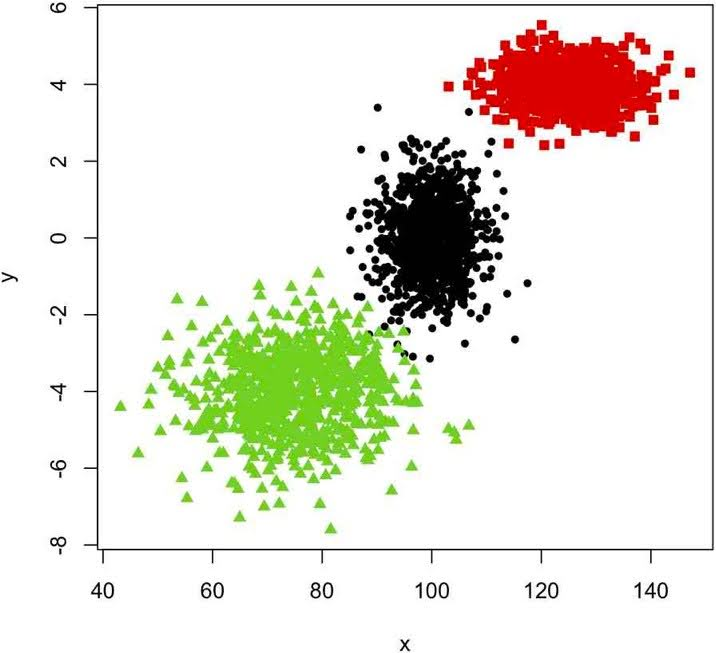
\includegraphics[width=0.95\textwidth,keepaspectratio]{images/dul/kmeans/k-means-example-1.jpg}
            \caption{Clusters.}
        \end{figure}
    \end{column}
\end{columns}

\framebreak

\begin{block}{}
    How to measure within-cluster variation? 

    \vspace{0.5em}

    The most common choice is squared Euclidean distance:
        \begin{equation}
            W(C_k) = \frac{1}{|C_k|} \sum_{i, i' \in C_k} \sum_{j=1}^{p} (x_{ij} - x_{i'j})^2
        \end{equation}
    
        where $|C_k|$ is the number of points in cluster $C_k$ and $x_{ij}$ is the $j^{th}$ feature of the $i^{th}$ point.
    
    \vspace{0.5em}
    
    Which means overall we solve:
        \begin{equation}
            \operatorname*{minimise}_{C_1, \ldots, C_k} \left\{ \sum_{k=1}^{K} \frac{1}{|C_k|} \sum_{i, i' \in C_k} \sum_{j=1}^{p} (x_{ij} - x_{i'j})^2 \right\}
        \end{equation}
\end{block}

\framebreak

\begin{itemize}
    \setlength{\itemsep}{0.5em}
    \item It turns out that this optimization problem is difficult to solve, as it is  discrete and there are nearly $K^n$	ways to split $n$ samples into $K$ clusters.
    \item In practice, use an iterative algorithm that finds a local minimum to this  optimization.
\end{itemize}

\framebreak

%pseudo code
\begin{algorithm}[H]
\caption{K-means Clustering Algorithm}
\KwIn{Dataset $D = \{x_1, x_2, \dots, x_n\}$, number of clusters $k$}
\KwOut{Cluster assignments for each data point}

\vspace{0.8em}

\textbf{Initialization:} Randomly initialize $k$ cluster centroids or seeds\;

\vspace{0.8em}

\textbf{Repeat until convergence:}
\begin{itemize}
    \item \textbf{Assignment Step:} Assign each data point $x_i$ to the nearest cluster based on a distance metric\;
    \vspace{0.5em}
    \item \textbf{Update Step:} Recompute cluster centroids using current assignments\;
    \vspace{0.5em}
    \item \textbf{Convergence Check:} Check if cluster assignments have changed or if centroids have stabilized\;
\end{itemize}

\vspace{0.8em}

\textbf{Return:} Final cluster assignments and centroids\;
\vspace{0.8em}

\end{algorithm}

\framebreak

\begin{center}
    Watch the K-means clustering algorithm in action:

    \vspace{1em}

    % \fetchconvertimageonly{https://i.ytimg.com/an_webp/2lZZ_FzlIJY/mqdefault_6s.webp?du=3000&sqp=CJLBvMEG&rs=AOn4CLBgJ_07yNkEYOFCkUraCWAH8Zmrsg}{images/thumbnails/k-means-youtube-thumbnail.png}
    \href{https://www.youtube.com/watch?v=2lZZ_FzlIJY}{%
    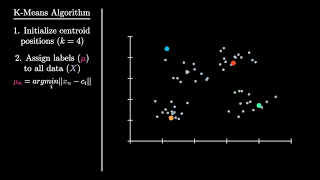
\includegraphics[width=0.95\textwidth,keepaspectratio]{images/thumbnails/k-means-youtube-thumbnail-0.png}
    }
    % \animategraphics[loop,controls,width=0.65\linewidth]{2}{images/gif_frames/k-mean-}{001}{014}
    % \includeGIF{images/k-mean-animation.gif}{k-mean}{0.95\linewidth}{12}
\end{center}

\framebreak

\begin{columns}
    \begin{column}{0.45\textwidth}
        \begin{enumerate}
            \setlength{\itemsep}{1em}
            \item It can be shown that the value of  the objective function will never  increase at each iteration of $k$-means.
            \item Since the algorithm finds local  minima, however, it will result in  different clusters with different  initializations.
        \end{itemize}
    \end{column}
    \begin{column}{0.55\textwidth}
        \begin{figure}
            \centering
            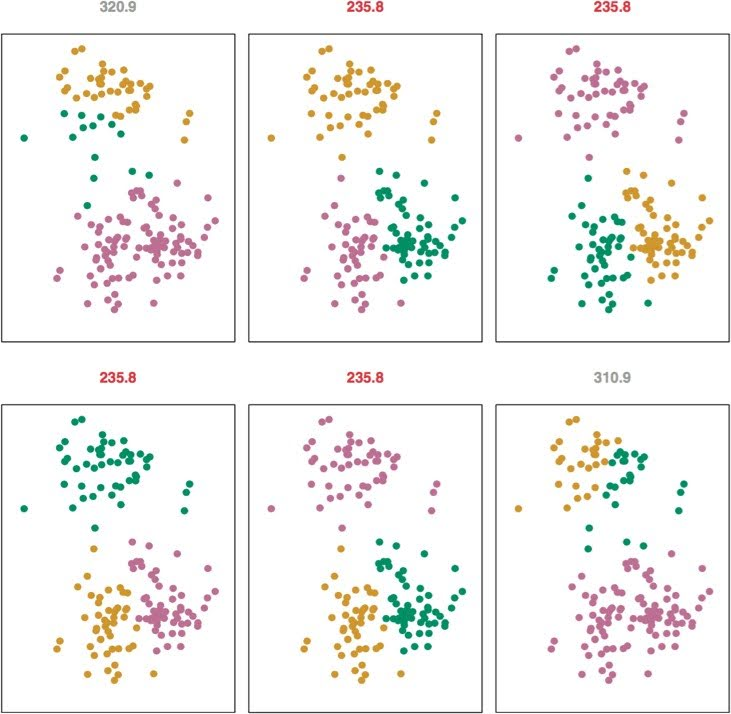
\includegraphics[width=\textwidth,keepaspectratio]{images/dul/kmeans/k-mean-different-init.jpg}
            \caption{Different initializations of K-means.}
        \end{figure}
    \end{column}
\end{columns}

\end{frame}

\begin{frame}[allowframebreaks]{K-means - Pros and Cons}
\begin{columns}
    \begin{column}{0.45\textwidth}
        \textbf{Pros}
        \begin{itemize}
            \setlength{\itemsep}{1em}
            \item Simple and easy to implement
            \item Efficient for large datasets
            \item Works well with spherical clusters
            \item Scalable to large datasets
        \end{itemize}
    \end{column}
    \begin{column}{0.55\textwidth}
        \textbf{Cons}
        \begin{itemize}
            \setlength{\itemsep}{1em}
            \item Not robust to data perturbations and different initializations
            \item Sensitive to initial centroid placement
            \item Assumes spherical clusters
            \item Requires specifying the number '$K$' of clusters in advance
            \item Sensitive to outliers
            \item May converge to local minima
            \item Not suitable for non-convex shapes
        \end{itemize}
    \end{column}
\end{columns}
\end{frame}
\begin{frame}[allowframebreaks]{Clustering - Hierarchical}
\begin{columns}
    \begin{column}{0.45\textwidth}
        Cluster based on distances  between observations.

        \vspace{0.8em}

        Represented as a tree hierarchy  (\textit{dendrogram}) rather than a  partition of data.

        \vspace{0.8em}

        Does not require committing to a  choice of $K$.
    \end{column}
    \begin{column}{0.55\textwidth}
        \begin{figure}
            \centering
            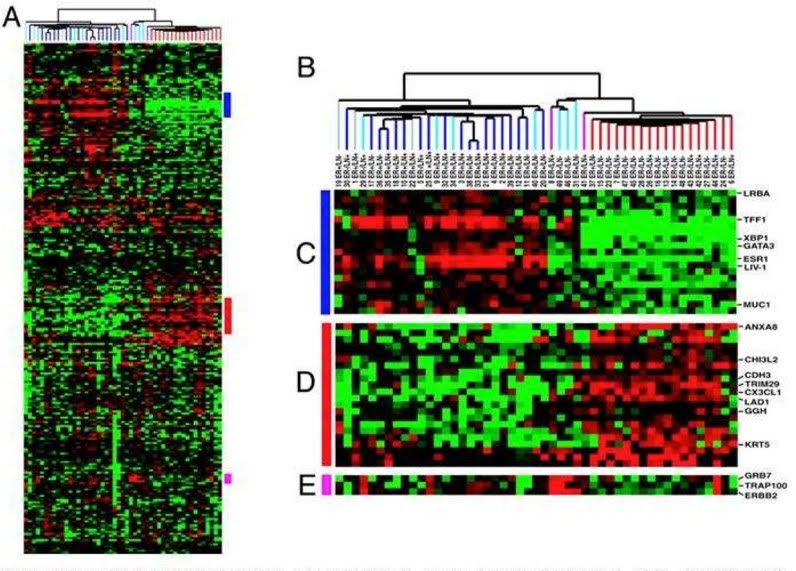
\includegraphics[width=0.8\textwidth,keepaspectratio]{images/dul/hierarchical/breast-tumor-subtypes.jpg}
            \caption{Sørlie, Therese, et al. (2003) "Repeated observation of breast  tumor subtypes in independent gene expression data sets," PNAS.}
        \end{figure}
    \end{column}
\end{columns}
\end{frame}

\begin{frame}[allowframebreaks]{Clustering - Hierarchical: Dendrograms}
\begin{columns}
    \begin{column}{0.45\textwidth}
        \begin{itemize}
            \setlength{\itemsep}{0.5em}
            \item Each leaf in a dendrogram is a sample/  observation.
            \item As we move up the dendrogram, observations  that are similar to each other begin to fuse  into branches.
            \item Branches then fuse into bigger branches.
            \item Observations that fuse later (near the top of  the tree, or root) are more different than observations that fuse earlier (near the leaves).
        \end{itemize}
    \end{column}

    \vspace{0.8em}

    \begin{column}{0.55\textwidth}
        \begin{figure}
            \centering
            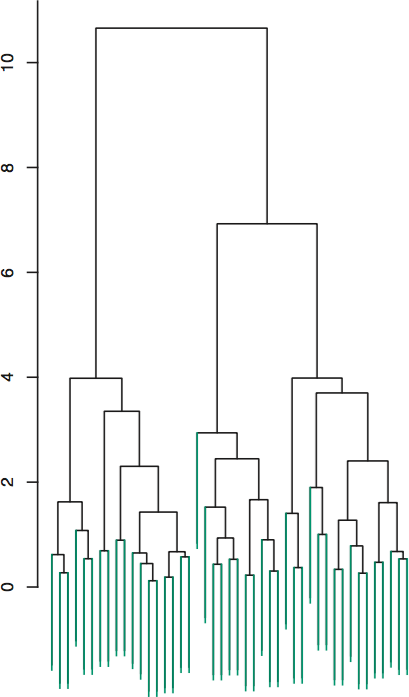
\includegraphics[width=0.95\textwidth,height=0.8\textheight,keepaspectratio]{images/dul/hierarchical/dendrograms.png}
            \caption{ISL (8th printing 2017)}
        \end{figure}
    \end{column}
\end{columns}

\framebreak

\begin{block}{}
    Note that the horizontal distance between observations on a  dendrogram is not the appropriate assessment of observation  similarity. Instead, look at vertical axis where branches are first fused.

    \vspace{1.5em}

    \begin{figure}
        \centering
        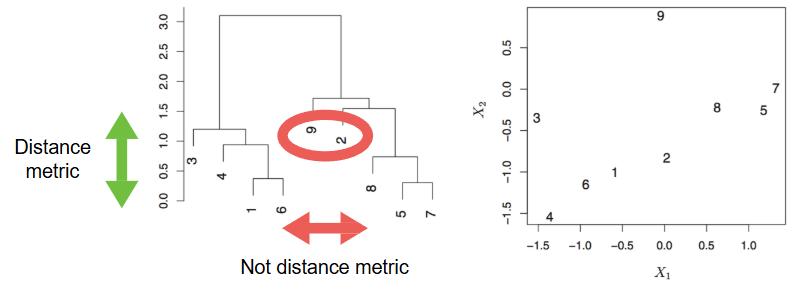
\includegraphics[width=0.95\textwidth,height=0.7\textheight,keepaspectratio]{images/dul/hierarchical/dendograms-distance-metric.png}
        \caption{ISL (8th printing 2017)}
    \end{figure}
\end{block}

\framebreak

\begin{columns}
    \begin{column}{0.45\textwidth}
        Clusters are created by  making a horizontal cut  across the dendrogram.  Clusters are the separate  trees below the cut.
    \end{column}

    \vspace{0.8em}

    \begin{column}{0.55\textwidth}
        \begin{figure}
            \centering
            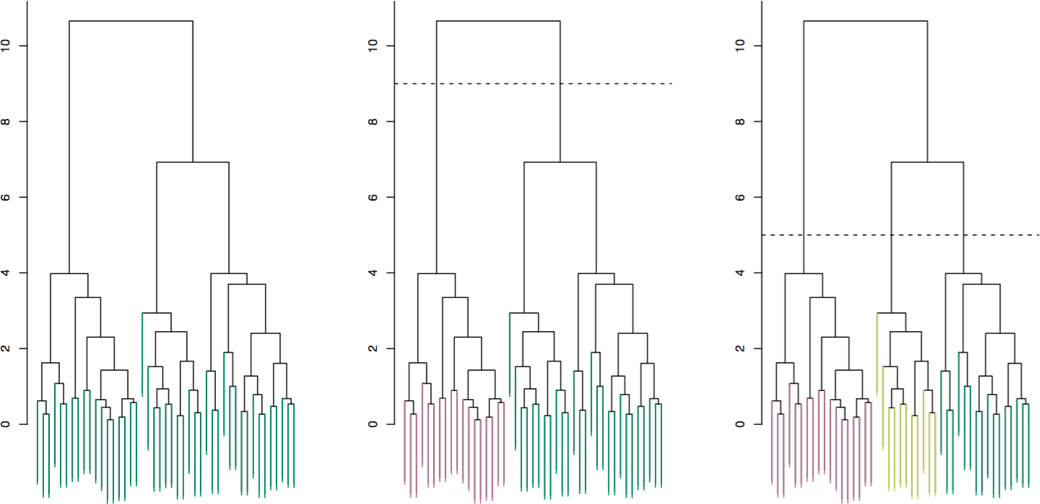
\includegraphics[width=1.05\textwidth,height=0.8\textheight,keepaspectratio]{images/dul/hierarchical/dendrograms-cluster.png}
            \caption{ISL (8th printing 2017)}
        \end{figure}
    \end{column}
\end{columns}

\framebreak

\begin{block}{Building a Dendrogram}
    A dendrogram is most commonly built using a bottom-up or agglomerative algorithm.

    \vspace{0.8em}

    We start at the leaves and group observations until we reach the root  containing the entire dataset.
    
    \vspace{0.8em}

    Like in $k$-means, we need a measure of similarity. Again, the most  common is Euclidean distance.

    \vspace{0.8em}

    \begin{itemize}
        \setlength{\itemsep}{0.5em}
        \item Compute the distance between each pair of observations.
        \item Merge the two closest observations into a cluster.
        \item Compute the distance between the new cluster and all other observations.
        \item Repeat until all observations are in one cluster.
        \item The distance between clusters is computed using a linkage method.
    \end{itemize}
\end{block}

\framebreak

% Hierarchical clustering Algorithm - pseudo code
\begin{algorithm}[H]
\caption{Hierarchical Clustering Algorithm}
\KwIn{Dataset $D = \{x_1, x_2, \dots, x_n\}$}
\KwOut{Dendrogram representing the hierarchical structure of clusters}
\textbf{Initialization:} Treat each data point as a separate cluster\;
\textbf{Compute distance matrix:} Calculate pairwise distances between all clusters\;
\textbf{Repeat until only one cluster remains:}
\begin{itemize}
    \item Find the two closest clusters based on the distance matrix\;
    \item Merge the two clusters into a new cluster\;
    \item Update the distance matrix to reflect the new cluster\;
    \item Recompute distances between the new cluster and all other clusters using a linkage method\;
\end{itemize}
\textbf{Return:} Dendrogram representing the hierarchical structure of clusters\;
\end{algorithm}

\href{https://www.w3schools.com/python/python_ml_hierarchial_clustering.asp}{w3schools: Codes and Playground}

\framebreak

\begin{figure}
    \centering
    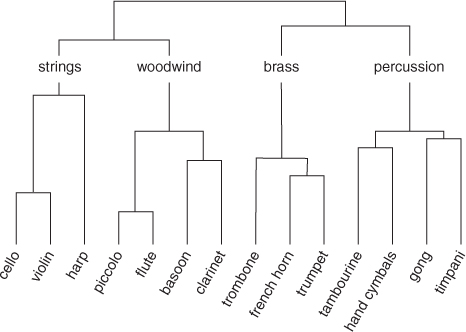
\includegraphics[width=0.95\textwidth,height=0.85\textheight,keepaspectratio]{images/dul/hierarchical/dendrogram-interpretation.png}
    \caption{Dendrogram interpretation.}
\end{figure}
\end{frame}


\begin{frame}[allowframebreaks]{Clustering - Hierarchical: Distance Metrics}
\vspace*{-2em}
\begin{block}{Distance between groups}
    It’s easy to compute Euclidean distance between two observations.  What is the distance or similarity between two groups or clusters of  observations?
    
    \vspace{0.8em}
    \textbf{Linkage}: defines the dissimilarity between two groups of observations.  Most common types are $complete$, $average$, $single$, and $centroid$.
\end{block}

\framebreak

\begin{itemize}
    \setlength{\itemsep}{0.5em}
    \item \textbf{Single Linkage}: Distance between two clusters is the minimum distance between any two points in the clusters.
    \item \textbf{Complete Linkage}: Distance between two clusters is the maximum distance between any two points in the clusters.
    \item \textbf{Average Linkage}: Distance between two clusters is the average distance between all pairs of points in the clusters.
    \item \textbf{Centroid Linkage}: Distance between two clusters is the distance between their centroids.
    \item \textbf{Ward's Linkage}: Distance between two clusters is the increase in variance when the two clusters are merged.
\end{itemize}

\framebreak

\begin{figure}
    \centering
    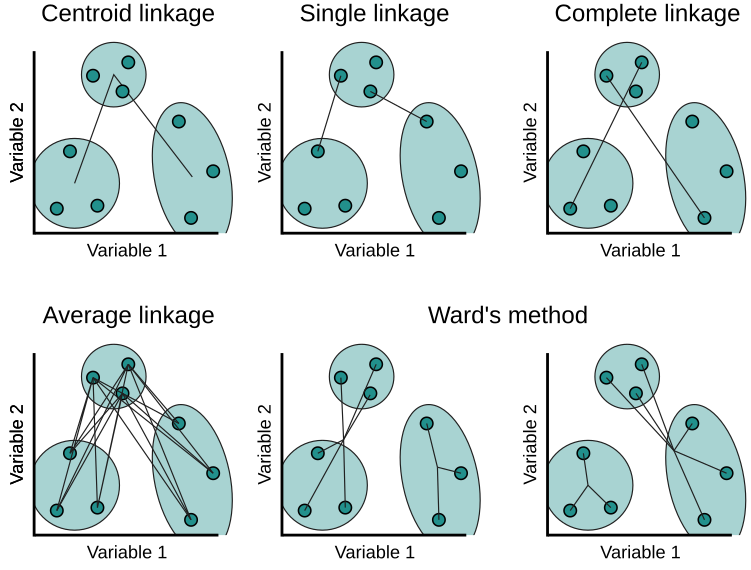
\includegraphics[width=0.95\textwidth,height=0.85\textheight,keepaspectratio]{images/dul/hierarchical/linkage.png}
    \caption{Linkage methods.}
\end{figure}

\begin{figure}
    \centering
    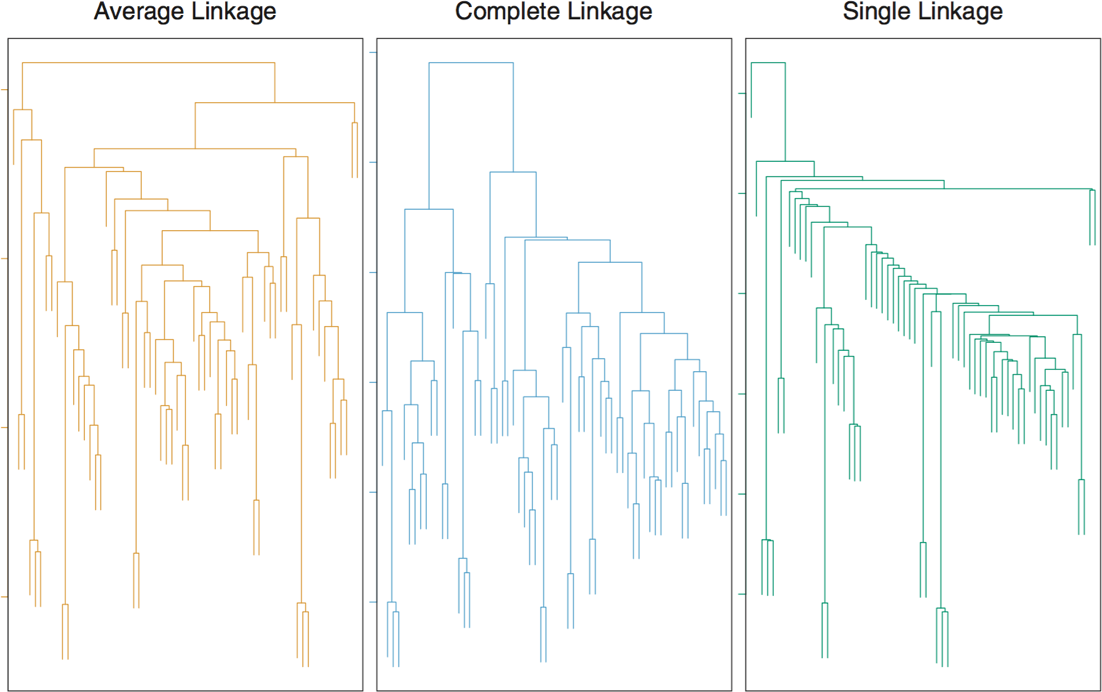
\includegraphics[width=0.95\textwidth,height=0.85\textheight,keepaspectratio]{images/dul/hierarchical/dendrogram-linkage-types.png}
    \caption{Dendrogram with different linkage types.}
\end{figure}
\end{frame}


\begin{frame}[allowframebreaks]{Clustering - Hierarchical: Pros and Cons}
\begin{columns}
    \begin{column}{0.5\textwidth}
        \textbf{Pros}
        \begin{itemize}
            \setlength{\itemsep}{1em}
            \item No need to specify the number of clusters $K$ in advance.
            \item Dendrograms provide a visual representation of the clustering process.
            \item Can capture complex cluster shapes and relationships.
        \end{itemize}
    \end{column}
    \begin{column}{0.5\textwidth}
        \textbf{Cons}
        \begin{itemize}
            \setlength{\itemsep}{1em}
            \item Computationally expensive for large datasets.
            \item Do have to pick where to cut the dendrogram to obtain clusters
            \item Sensitive to similarity measure and type of linkage used.
            \item Sensitive to noise and outliers.
            \item Difficult to interpret and choose the optimal number of clusters.
        \end{itemize}
    \end{column}
\end{columns}
\end{frame}

% Density-Based Spatial Clustering of Applications with Noise
\begin{frame}[allowframebreaks]{Clustering - Density-Based Methods}
\begin{itemize}
    \setlength{\itemsep}{0.1em}
    \item Clustering based on density (local cluster criterion), such as density-connected points or based on an explicitly constructed density function.
    \item \textbf{Major features}:
    \begin{itemize}
        \item Discover clusters of arbitrary shape
        \item Handle noise
        \item One scan
        \item Need density parameters
    \end{itemize}

    \framebreak
    
    \item \textbf{Major algorithms}:
    \begin{itemize}
        \item DBSCAN (Density-Based Spatial Clustering of Applications with Noise): Ester, et al. (KDD’96)
        \item OPTICS (Ordering Points to Identify the Clustering Structure): Ankerst, et al. (SIGMOD’99)
        \item HDBSCAN (Hierarchical Density-Based Spatial Clustering of Applications with Noise): Campello, et al. (ACM TIST’15)
        \item DENCLUE (DENsity-based CLUstEring): Hinneburg and Gabriel (KDD’97)
        \item CLIQUE (CLustering In QUEst): Karypis, Han, and Kumar (SIGMOD’98)
    \end{itemize}
\end{itemize}
\end{frame}

\begin{frame}[allowframebreaks]{Clustering - DBSCAN}
\begin{itemize}
    \item \textbf{DBSCAN} (Density-Based Spatial Clustering of Applications with Noise):
    \begin{itemize}
        \item Density = number of points within a specified radius $\epsilon$.
        \item A point is a core point if it has more than a specified number of points (MinPts) within $\epsilon$. These are points that are at the interior of a cluster.
        \item A border point has fewer than MinPts within $\epsilon$, but is in the neighborhood of a core point
        \item A noise point is any point that is not a core point or a border point.
        \item Groups together points that are closely packed together, marking as outliers points that lie alone in low-density regions.
        \item Parameters:
        \begin{itemize}
            \item $\epsilon$: Maximum distance between two points for them to be considered as in the same neighborhood.
            \item MinPts: Minimum number of points required to form a dense region.
        \end{itemize}
    \end{itemize}
\end{itemize}

\framebreak

\begin{figure}
    \centering
    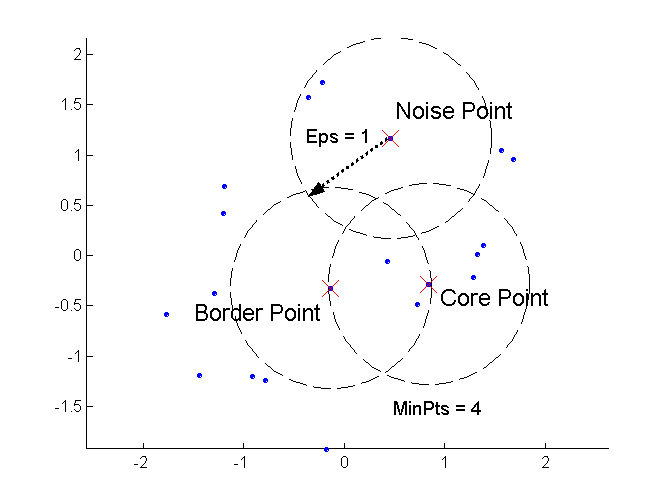
\includegraphics[width=0.95\textwidth,height=0.8\textheight,keepaspectratio]{images/dul/dbscan/dbscan-features.png}
    \caption{DBSCAN features: Core, Border, and Noise Points}
\end{figure}
\end{frame}


\begin{frame}[allowframebreaks]{Clustering - DBSCAN: Algorithm}
\begin{algorithm}[H]
\caption{Graph-Based DBSCAN Clustering}
\KwIn{Set of points $P$, distance threshold $\varepsilon$, minimum number of points $minPts$}
\KwOut{A set of clusters}

Construct a directed graph $G = (V, E)$ where each node in $V$ corresponds to a point in $P$\;

\ForEach{point $c \in P$}{
    \If{$c$ is a core point (i.e., $|\mathcal{N}_\varepsilon(c)| \geq minPts$)}{
        \ForEach{point $p \in \mathcal{N}_\varepsilon(c)$}{
            Add a directed edge $(c \rightarrow p)$ to $E$\;
        }
    }
}

$N \leftarrow V$\;

\While{there exists a core point $c \in N$}{
    Let $X$ be the set of nodes reachable from $c$ via directed edges in $G$\;
    Form a cluster $C = X \cup \{c\}$\;
    Remove all nodes in $C$ from $N$\;
}

\end{algorithm}
\end{frame}

\begin{frame}[allowframebreaks]{Clustering - DBSCAN: Core, Border, and Noise Points}
\begin{columns}
    \begin{column}{0.5\textwidth}
       \begin{figure}
            \centering
            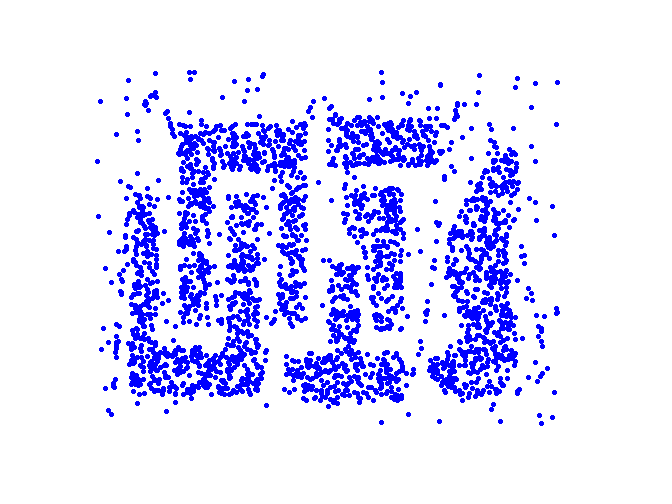
\includegraphics[width=1.2\textwidth,keepaspectratio]{images/dul/dbscan/dbscan-original-pts-1.png}
            \caption{Original Points}
        \end{figure}
    \end{column}
    \begin{column}{0.5\textwidth}
        \begin{figure}
            \centering
            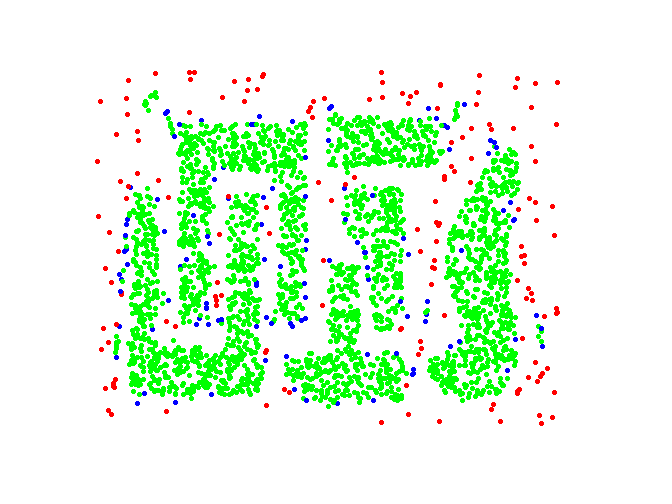
\includegraphics[width=1.2\textwidth,keepaspectratio]{images/dul/dbscan/dbscan-core-border-noise.png}
            \caption{Point types: \textcolor{green}{Core}, \textcolor{blue}{Border}, and \textcolor{red}{Noise} Points}
        \end{figure}
    \end{column}
\end{columns}

\begin{center}
Eps = 10, MinPts = 4
\end{center}

\end{frame}

\begin{frame}[allowframebreaks]{When DBSCAN Works Well}
\begin{columns}
    \begin{column}{0.5\textwidth}
       \begin{figure}
            \centering
            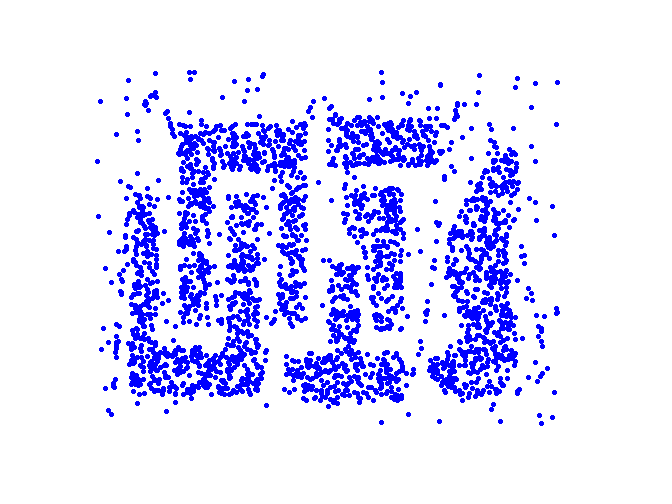
\includegraphics[width=1\textwidth,keepaspectratio]{images/dul/dbscan/dbscan-original-pts-1.png}
            \caption{Original Points}
        \end{figure}
    \end{column}
    \begin{column}{0.5\textwidth}
        \begin{figure}
            \centering
            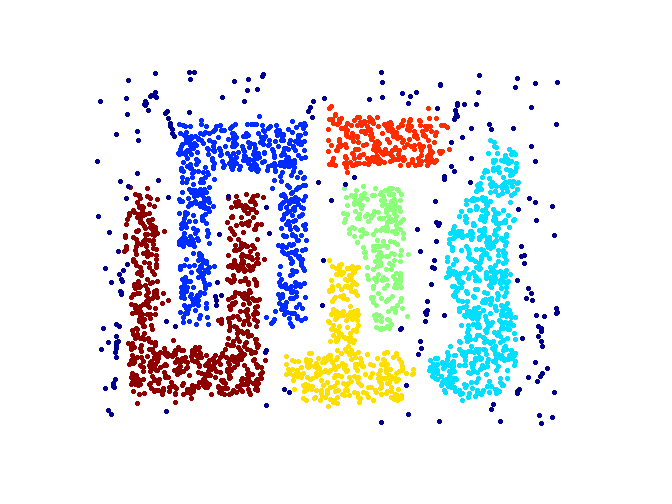
\includegraphics[width=1\textwidth,keepaspectratio]{images/dul/dbscan/dbscan-clusters.png}
            \caption{Clusters identified by DBSCAN}
        \end{figure}
    \end{column}
\end{columns}

DBSCAN works well when:
\begin{itemize}
        \item Clusters are of varying shapes and sizes.
        \item There is a clear distinction between dense and sparse regions.
        \item The data contains noise or outliers.
\end{itemize}
\end{frame}

\begin{frame}[allowframebreaks]{When DBSCAN Doesn't Works Well}
\begin{columns}
    \begin{column}{0.5\textwidth}
       \begin{figure}
            \centering
            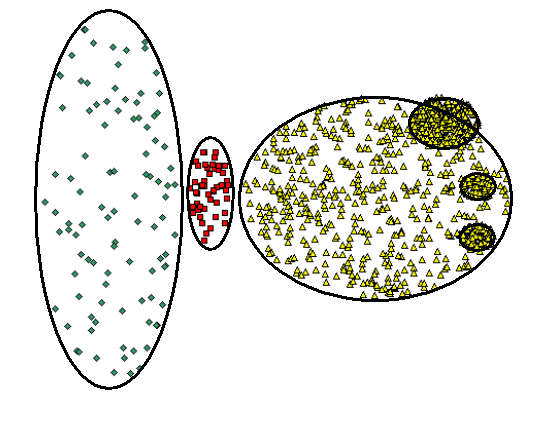
\includegraphics[width=0.9\textwidth,keepaspectratio]{images/dul/dbscan/dbscan-original-pts-2.png}
            \caption{Original Points}
        \end{figure}

        DBSCAN does not work well when:
        \begin{itemize}
            \item Clusters are of varying densities.
            \item The data has varying scales or dimensions.
            \item There are overlapping clusters.
            \item The choice of $\epsilon$ and MinPts is not suitable for the data distribution.
        \end{itemize}
    \end{column}
    \begin{column}{0.5\textwidth}
        \begin{figure}
            \centering
            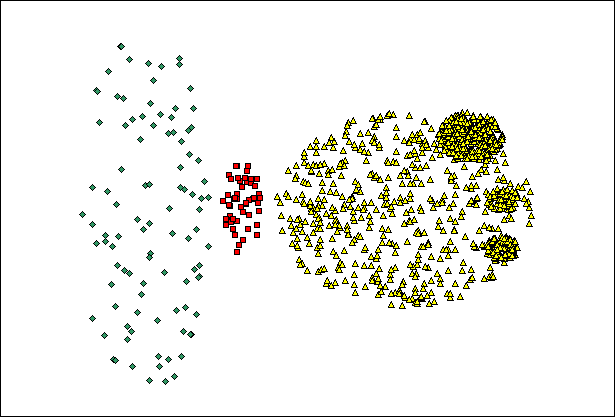
\includegraphics[width=0.9\textwidth,keepaspectratio]{images/dul/dbscan/dbscan-clusters-1.png}
            \caption{MinPts=4, $\epsilon$=9.75}
        \end{figure}
        \begin{figure}
            \centering
            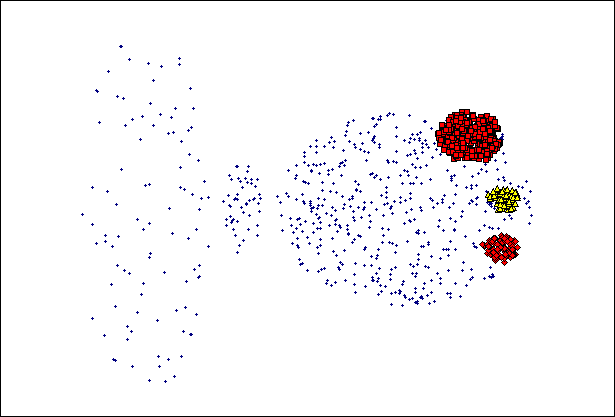
\includegraphics[width=0.9\textwidth,keepaspectratio]{images/dul/dbscan/dbscan-clusters-2.png}
            \caption{MinPts=4, $\epsilon$=9.92}
        \end{figure}
    \end{column}
\end{columns}

\end{frame}

\begin{frame}[allowframebreaks]{DBSCAN: Determining $\epsilon$ and MinPts}
\begin{itemize}
    \item A common approach to determine $\epsilon$ is to use a k-distance graph:
    \begin{itemize}
        \item For each point, compute the distance to its k-th nearest neighbor.
        \item Plot these distances in ascending order.
        \item Look for a "knee" in the plot, which indicates a suitable value for $\epsilon$.
    \end{itemize}
    \item MinPts is often set based on domain knowledge or heuristics:
    \begin{itemize}
        \item A common rule of thumb is to set MinPts to at least the dimensionality of the data plus one (e.g., for 2D data, MinPts = 3).
        \item Higher values of MinPts can lead to fewer clusters and more noise points.
    \end{itemize}
\end{itemize}

\begin{figure}
    \centering
    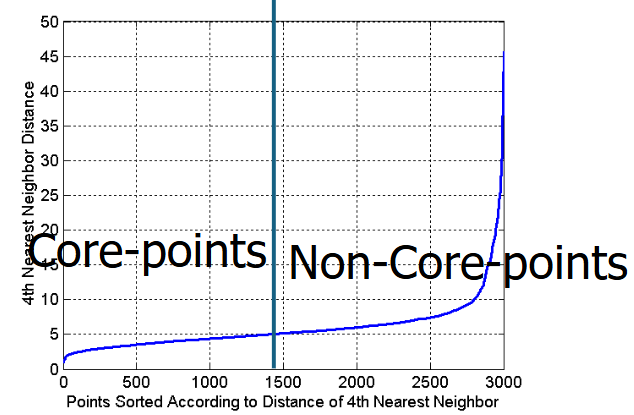
\includegraphics[height=0.8\textheight,keepaspectratio]{images/dul/dbscan/eps-determination.png}
    \caption{Run K-means for Minp=4 and not fixed $\epsilon$}
\end{figure}
\end{frame}


\begin{frame}[allowframebreaks]{DBSCAN: Complexity and Limitations}
\begin{itemize}
    \item \textbf{Complexity}:
    \begin{itemize}
        \item The time complexity of DBSCAN is $O(n \log n)$ for spatial data structures like KD-trees or R-trees, where $n$ is the number of points.
        \item Without spatial indexing, the complexity can degrade to $O(n^2)$.
        \item Space complexity is $O(n)$, as it needs to store the points and their cluster assignments.
    \end{itemize}
    \item \textbf{Limitations}:
    \begin{itemize}
        \item Sensitive to the choice of $\epsilon$ and MinPts parameters.
        \item Struggles with clusters of varying densities.
        \item Not suitable for high-dimensional data due to the curse of dimensionality.
        \item Cannot handle clusters that are not well-separated in terms of density.
    \end{itemize}
\end{itemize}
\end{frame}


\begin{frame}[allowframebreaks]{DBSCAN: Summary}
\begin{itemize}
    \item \textbf{Good}:
    \begin{itemize}
        \item Can discover clusters of arbitrary shape.
        \item Effectively handles noise and outliers.
        \item Requires only one scan of the data.
        \item Suitable for datasets with varying densities.
        \item Does not require prior knowledge of the number of clusters.
    \end{itemize}
    \item \textbf{Bad}:
    \begin{itemize}
        \item Does not work well in high-dimensional datasets.
        \item Parameter selection is tricky.
        \item Has problems identifying clusters of varying densities (\textrightarrow{} SSN algorithm).
        \item Density estimation is simplistic (\textrightarrow{} does not create a real density function, but rather a graph of density-connected points).
    \end{itemize}
\end{itemize}
\end{frame}


\begin{frame}[allowframebreaks]{DBSCAN: Algorithm Revisited}
\begin{figure}
    \centering
    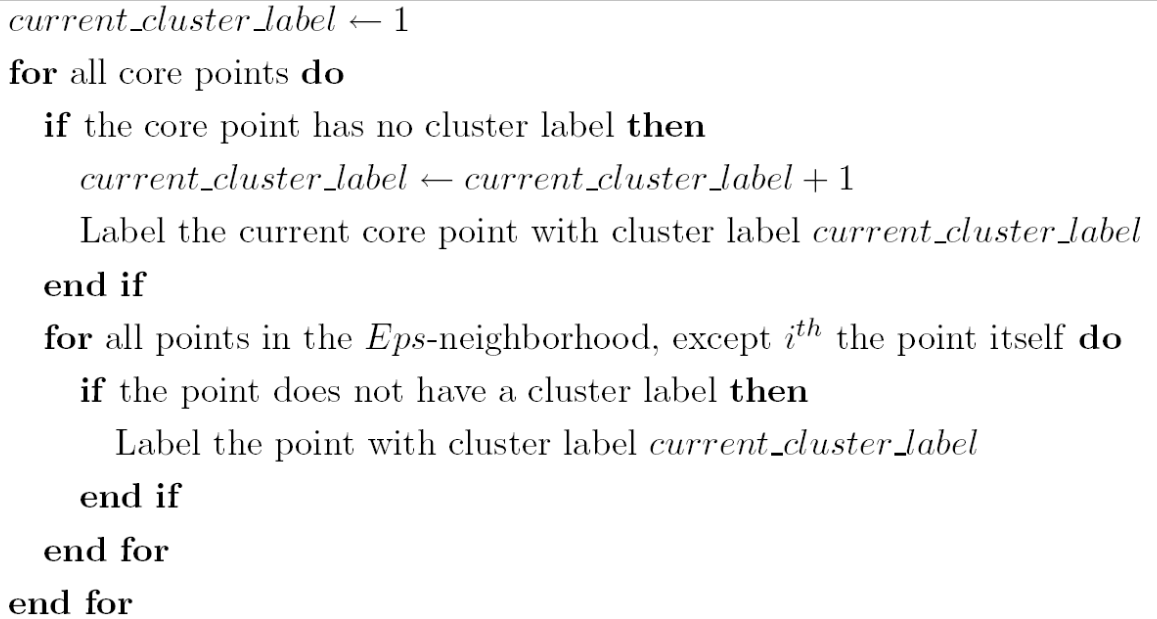
\includegraphics[height=0.75\textheight,keepaspectratio]{images/dul/dbscan/algorithm.png}
    \caption{DBSCAN Algorithm Steps}
\end{figure}
\end{frame}